% History
% 12/06/2024  (岸)	修論下書き用texファイル作成
% 12/12/2024  (岸)	フォントサイズを11pt, 行間を1.5に設定
% コンパイルの仕方
% 		uplatex chapter1_v1.tex
% 		upbibtex chapter1_v1
% 		uplatex chapter1_v1.tex
% 		uplatex chapter1_v1.tex
% 		dvipdfmx chapter1_v1.dvi

% フォントサイズを11ptに設定
\documentclass[a4paper,11pt,nomag]{jsreport}

\usepackage[dvipdfm,truedimen]{geometry}
\geometry{top=22mm,bottom=22mm,left=22mm,right=22mm}
%% jsclasses系で文字サイズ11pt や 12pt をクラスオプションに指定すると,
%% 長さが拡大されるため,nomagオプションを併用している.
%% https://oku.edu.mie-u.ac.jp/~okumura/jsclasses/ のFAQをよく読むこと.

%\usepackage{layout}
%\usepackage[utf8]{inputenc} %不要かも
\usepackage[T1]{fontenc} %utf8フォントエンコーディング指定
\usepackage{lmodern} % 11pt, nomag を使っているので
% CloudLaTeX の場合は下の1行を有効にすること
% \AtBeginDvi{\special{pdf:mapfile ptex-ipaex.map}}
\usepackage{array}
\newcommand{\bhline}[1]{\noalign{\hrule height #1}}  
\newcommand{\bvline}[1]{\vrule width #1}
\renewcommand{\baselinestretch}{1.5} % 教授が赤修正を入れやすいように行間を1.5に設定
\usepackage[subrefformat=parens]{subcaption}
\usepackage[dvipdfmx]{graphicx} % dvipdfmx を前提としている
\usepackage[dvipdfmx]{color}
\usepackage{caption}
\usepackage{subcaption}
\usepackage{bbm}
\usepackage{multirow}
\usepackage{arydshln}
\usepackage{here} % 図表の位置決め用
\usepackage{amsmath,amssymb}% 数式用
\usepackage{url}      % URL等記載用.\verbより便利
\usepackage{enumerate}
\usepackage{midpage}

% サブキャプションのフォーマットを調整
\renewcommand\thesubfigure{(\alph{subfigure})}
\captionsetup[subfigure]{labelformat=simple, labelsep=space}

\begin{document}

\chapter*{深層学習を用いた動物分類に関する既存研究}

\setcounter{chapter}{1}
\section{赤外線画像に対する既存研究}

hoge \cite{schneider2020}

% \begin{figure}[tbp]
%   \centering
%   \begin{subfigure}[b]{0.45\linewidth}
%     \centering
%     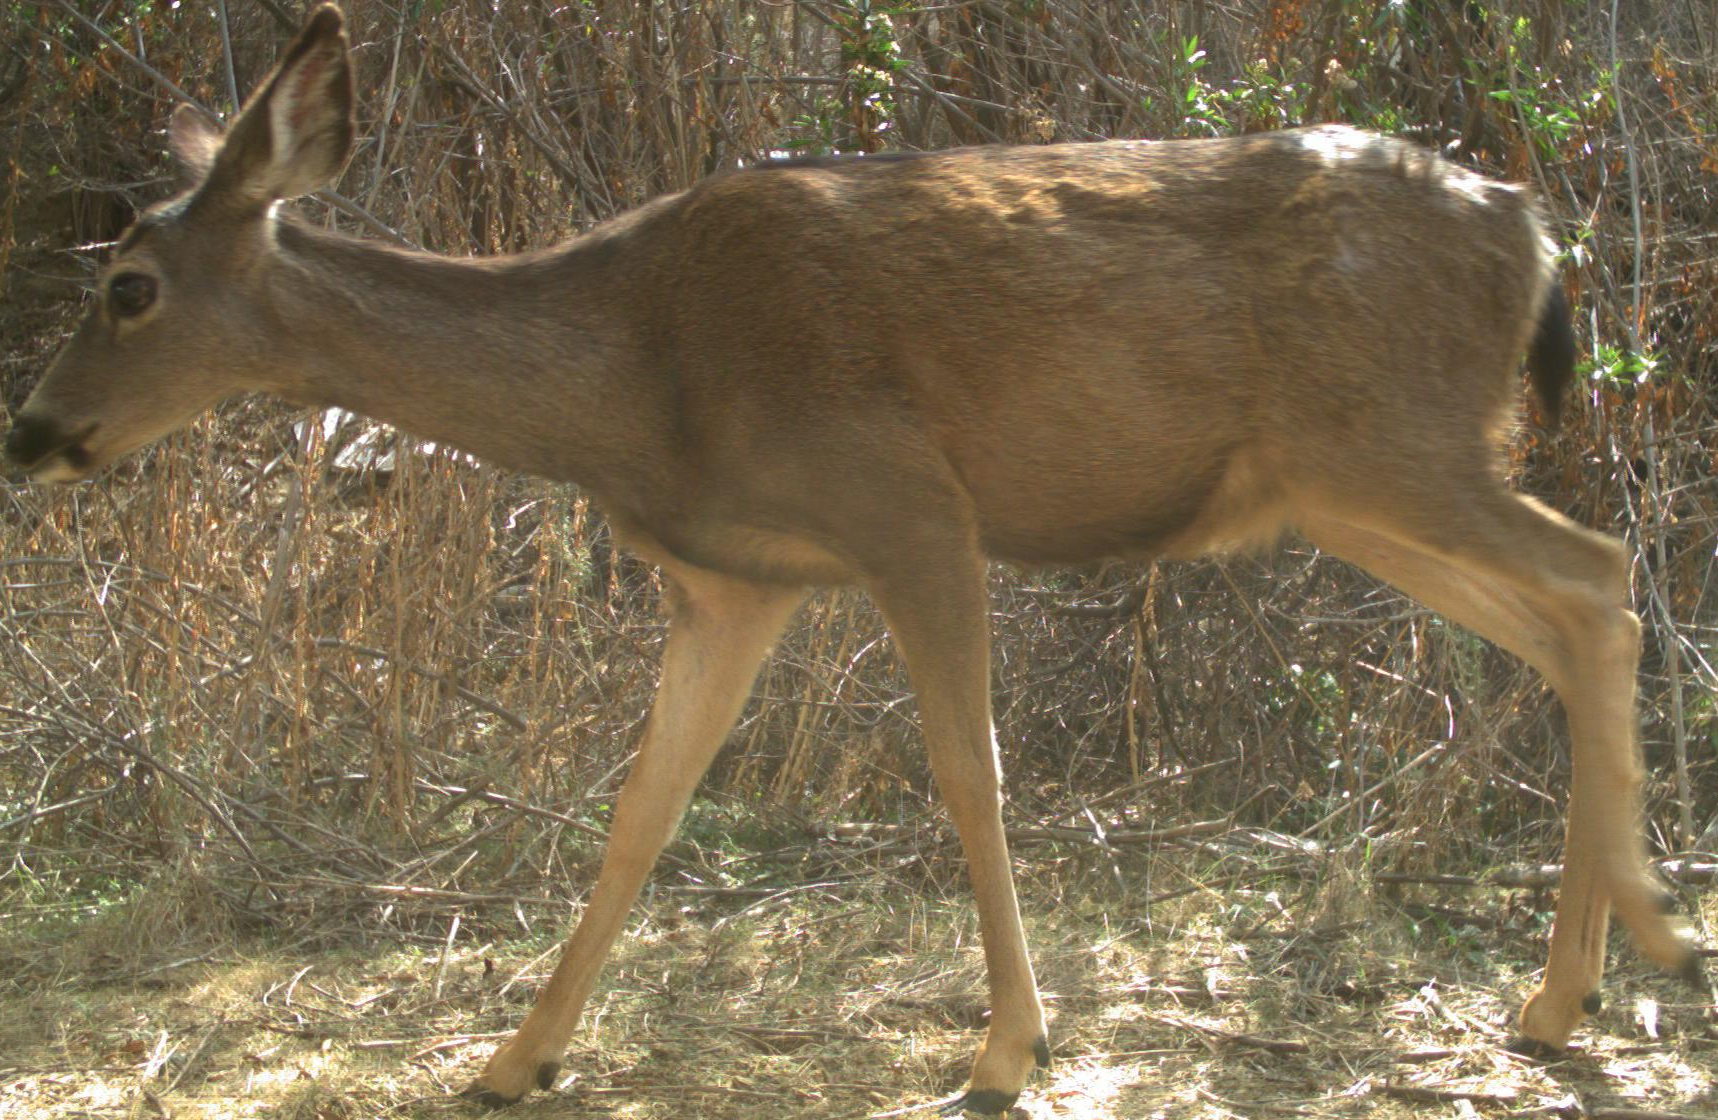
\includegraphics[height=0.7\linewidth, keepaspectratio]{cct_color_deer.png}
%     \caption{可視光画像}
%     \label{fig:color_deer}
%   \end{subfigure}
%   \hfill
%   \begin{subfigure}[b]{0.45\linewidth}
%     \centering
%     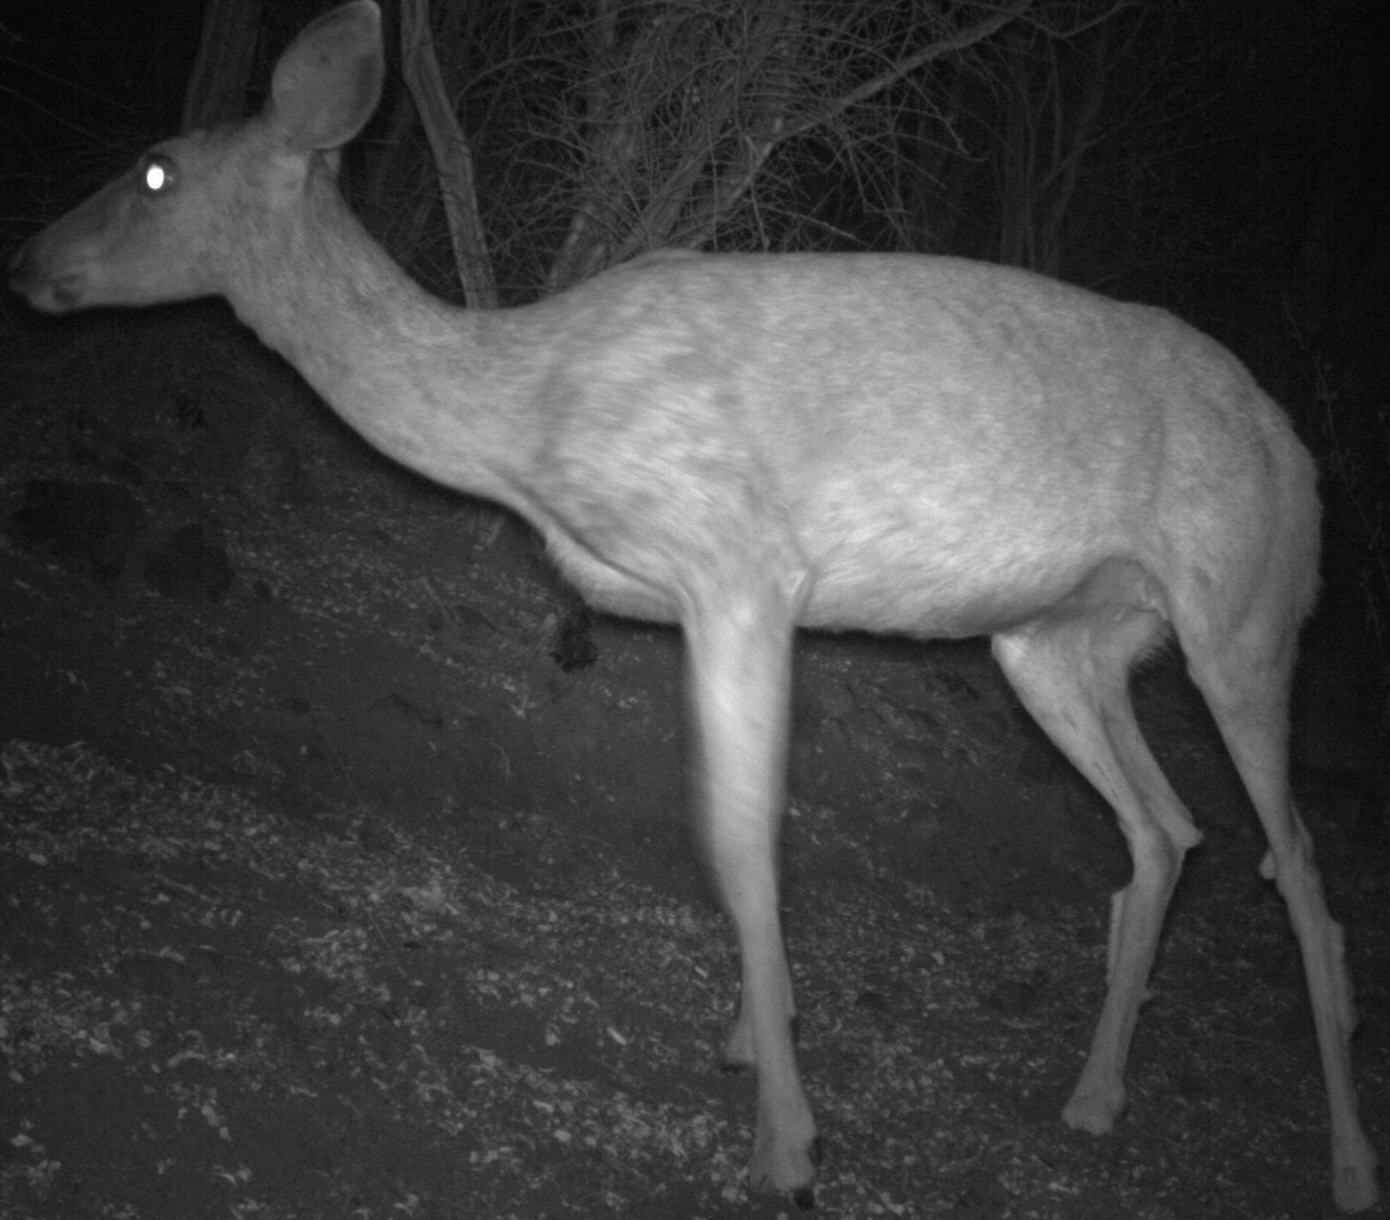
\includegraphics[height=0.7\linewidth, keepaspectratio]{cct_infrared_deer.png}
%     \caption{赤外線画像}
%     \label{fig:infrared_deer}
%   \end{subfigure}
%   \caption{撮影方法の違いによる物体の写り方}
%   \label{fig:camera}
% \end{figure}

\subsection{Few-Shot Open-Set Recognitionに関する既存研究}

hogehoge \cite{peeler}

% ここから参考文献bibtexの設定
\bibliographystyle{kishiIEEEtr}
\bibliography{references}

\end{document}